\begin{figure}[h]
    \centering
    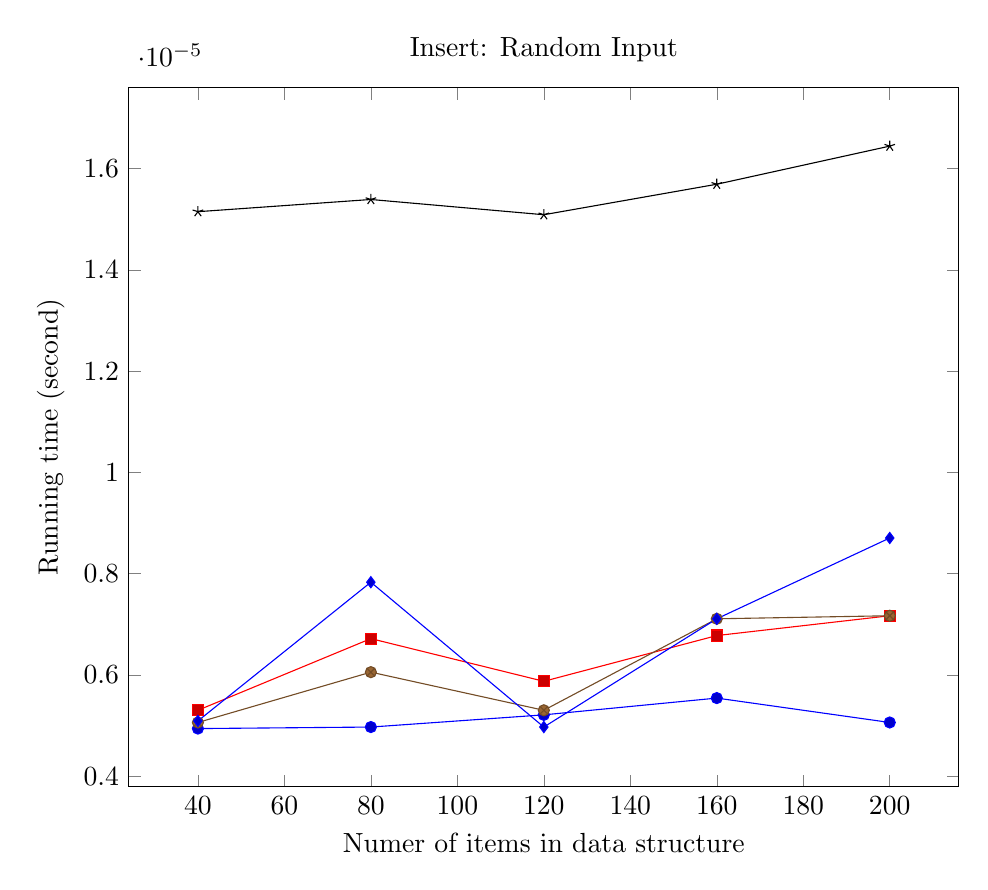
\begin{tikzpicture}
        \begin{axis}[
            xlabel={Numer of items in data structure},
            ylabel={Running time (second)},
            title={Insert: Random Input},
            width=\textwidth
        ]
		\addplot coordinates {
			(40, 4.939275522986008e-06)
			(80, 4.9693930566974135e-06)
			(120, 5.210333325678107e-06)
			(160, 5.541626196148286e-06)
			(200, 5.059745657476355e-06)
		};
		\addplot coordinates {
			(40, 5.300685926812321e-06)
			(80, 6.71621000982725e-06)
			(120, 5.872919066618465e-06)
			(160, 6.776445076894788e-06)
			(200, 7.167973014432505e-06)
		};
		\addplot coordinates {
			(40, 5.059745657476355e-06)
			(80, 6.053624268886892e-06)
			(120, 5.300685926812321e-06)
			(160, 7.107737947364967e-06)
			(200, 7.167973014787777e-06)
		};
		\addplot coordinates {
			(40, 1.5149119438717661e-05)
			(80, 1.5390059708053626e-05)
			(120, 1.5088884371294853e-05)
			(160, 1.5691235044812402e-05)
			(200, 1.6444173386531702e-05)
		};
		\addplot coordinates {
			(40, 5.089863190832488e-06)
			(80, 7.830558755372864e-06)
			(120, 4.969393056342142e-06)
			(160, 7.107737947364967e-06)
			(200, 8.703967231937782e-06)
		};
        \legend{}
        \end{axis}
    \end{tikzpicture}
    \caption{Average of 0 operations, benchmarked every 0, starting at 0.}
\end{figure}